\documentclass[hyperref={colorlinks, citecolor=blue}]{beamer}
\usepackage{float,times,graphicx,mathtools}
\usepackage{amsmath}
\usepackage{amsfonts}
\usepackage{amssymb}
\usepackage{latexsym}
\usepackage{epsfig}
\usepackage{graphicx}
\usepackage{color}
\usepackage{pdfpages}
\usepackage{natbib}
\usepackage{setspace}
\usepackage{multirow}
\usepackage{bbm}
\usepackage{MnSymbol,wasysym}
\usepackage{tensor}
\usepackage{tikz}

\usetikzlibrary{arrows,decorations.pathmorphing,backgrounds,positioning,fit,petri,calc,shadows, quotes}

\setbeamertemplate{caption}{\raggedright\insertcaption\par}
\usefonttheme{serif}
\onehalfspacing

\title{Incorporating Mortality Estimation into Population Reconstruction}

\begin{document}

\frame{\titlepage}

\begin{frame}
\frametitle{Brief Introduction to Mortality Modelling}
Let $T$ be the time (number of years) to death of a newborn (i.e. aged $0$), we have
\begin{align*}
_tq_x = P(T \leq t+x | T > x),
\end{align*}
 i.e. the probability that the newborn will die \textit{within} $t$ years given that she has survived for $x$ years, then 
\begin{align*}
_tp_x = 1 - \, _tq_x = P(T \geq t+x | T > x)
\end{align*}
 is the probability that an individual aged $x$ will survive \textit{at least} $t$ years.
\end{frame}

\begin{frame}
\frametitle{Brief Introduction to Mortality Modelling}
Some common demographic measures:
\begin{itemize}
\item $_{5}q_{0}$ : child mortality, i.e. probability of a newborn dying \textit{within} $5$ years, before reaching age $5$
\item $_{45}q_{15}$ : adult mortality, i.e. probability of an individual aged $15$ dying \textit{within} $45$ years, before reaching age $60$
\end{itemize}
\end{frame}

\begin{frame}
\frametitle{Force of Mortality \textit{vs} Death Probabilities}
Force of mortality is defined as:
\begin{align*}
\mu_{x+t} &= \lim_{\delta t \to 0} \frac{P(T \leq x+t+\delta t	| T > x+t)}{\delta t},	\\
					&= - \frac{1}{\tensor[_t]{p}{_x}}\frac{d}{dt} \tensor[_t]{p}{_x}, \\
					&= -\frac{d}{dt} \log \tensor[_t]{p}{_x}, \\
					\implies \tensor[_t]{q}{_x} &= 1- \tensor[_t]{p}{_x} = 1 - e^{- \int^t_0 \mu_{x+s} \, ds}.
\end{align*}
Intuitively it can be thought as a measure of the instantaneous ``death probability'' at age $x+t$. 
\begin{itemize}
\item the force of mortality is a \textit{rate}, $\mu \in [0, \infty)$
\item the death probability is a \textit{probability}, $\q \in [0, 1]$
\end{itemize}
\end{frame}

\begin{frame}
\frametitle{Central Mortality Rates}
It is often impossible to model directly on $\mu$. \\~\\

A usual practice is to aggregate data into separate age groups (usually 1 year), with mortality measured by the \textit{central mortality rates}:
\begin{align*}
_1m_{x} = m_x = \frac{\int^1_0 E_{x+t} \mu_{x+t} \,dt}{\int^1_0 E_{x+t} \,dt} = \frac{\mathbbm{E}(_1d_x)}{_1E^C_x}
\end{align*}
where $_1E^C_x$ and $_1d_x$ are the central exposures and number of deaths in age $[x, x+1)$ in 1 year. 
\begin{itemize}
\item Intuitively the central mortality rate can be viewed as the average force of mortality weighted by the corresponding exposures
\item Most mortality modelling is done on $m_x$.
\end{itemize}
\end{frame}

\begin{frame}
\frametitle{Conversion between $\mu_x$, $m_x$ and $q_x$}
As mentioned before, the exact relationship between $\mu_x$ and $q_x$ is $\tensor[_t]{q}{_x} &= 1 - e^{- \int^t_0 \mu_{x+s} \, ds}$, however, this requires integration over the age range. Often simplifying assumptions are made, two common ones are:
\begin{itemize}
\item[1)] Constant force of mortality $\rightarrow$ the force of mortality is constant within the age group \\
$\implies {q}{_x}  = 1 - e^{-\mu_{x+0.5}} \approx 1 - e^{-m_x}$
\item[2)] Uniform distribution of deaths $\rightarrow$ deaths are uniformly distributed over the age range \\
$\implies {q}{_x} = \frac{m_x}{1 + 0.5 m_x}$
\end{itemize}
\end{frame}

\begin{frame}
\frametitle{Mortality Models}
Recall 
\begin{align*}
m_x = \frac{\mathbbm{E}(d_x)}{E^C_x} \implies \mathbbm{E}(d_x) = E^C_x \, m_x
\end{align*}
Since $d_x$ is a count variable, it is often modelled as Poisson distributions, i.e. $d_x \sim Poisson(E^C_x \, m_x)$. Alternatives include
\begin{itemize}
\item $d_x \sim Binomial(E^0_x, q_x), $ where $E^0_x$ is the initial exposures
\item $\log(m_x) \sim N(\log(\hat{m_x}), \sigma), $ where $\hat{m_x}$ is the crude mortality rates

\item the Poisson distribution is often too restrictive as $Var(d_x) = \mathbbm{E}(d_x)$, and over-dispersion usually presents in mortality data.
\begin{itemize}
\item[\hookrightarrow] introduce an extra parameter of specific form to capture the excessive variance, one arrives at a Negative Binomial distribution, i.e. $d_x \sim NegBinom(E^C_x \, m_x, s)$
\end{itemize}
\end{itemize}
\end{frame}

\begin{frame}
\frametitle{Mortality Models}
Typical non-HIV infected mortality schedules, England and Wales males and females \footnote[frame]{Data obtained from the Office for National Statistics}
\newline
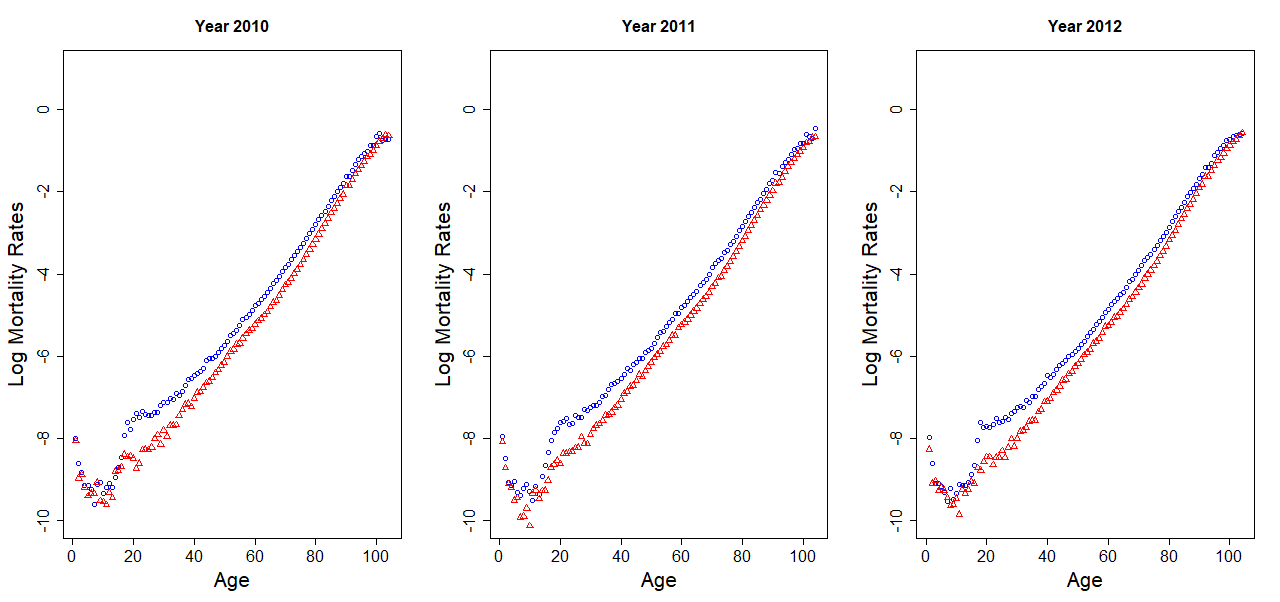
\includegraphics[width=\linewidth]{Graphs/crude mort rates.png}
\end{frame}

\begin{frame}
\frametitle{Mortality Models}
\begin{columns}
\begin{column}{0.4\linewidth}
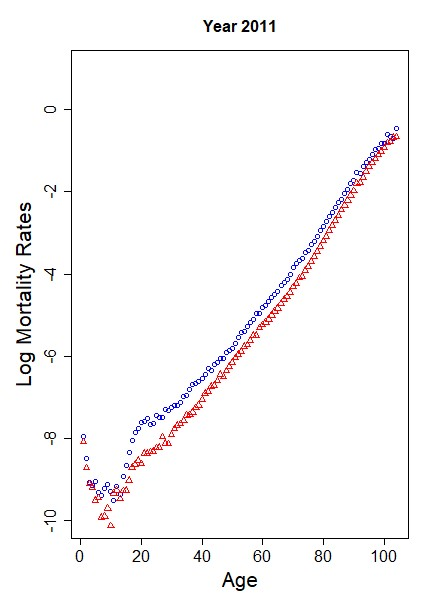
\includegraphics[width=\linewidth]{Graphs/crude mort rates 2011.jpg}
\end{column}
\begin{column}{0.7\linewidth}
\begin{itemize}
\item male mortality (blue) is higher than female mortality (red) most of the time
\item infant mortality is exceptionally high, followed by a sharp decrease into early teens
\item humps can be observed at late teens to early adulthood, more prominent for males (accident hump / maternal hump)
\item mortality increases steadily and relatively log-linearly after the mortality humps into older ages due to senescence
\end{itemize}
\end{column}
\end{columns}
\end{frame}

\begin{frame}
\frametitle{Mortality Models}
One of the earliest attempts in mortality modelling dates back to 1825, the Gompertz law of mortality \citep{gompertz1825on},
\begin{align*}
\log (m_x) = a + bx,
\end{align*}
which is then modified to the Gompertz-Makeham law \citep{makeham1860law} with the addition of an age invariant background mortality constant (age-unrelated deaths such as accidents)
\begin{align*}
m_x = A + BC^x
\end{align*}
\begin{itemize}
\item relatively simple, with only few parameters
\item provides adequate fit to mortality at older ages
\item only applicable to older ages, due to the log-linearity assumption
\end{itemize}
\end{frame}

\begin{frame}
\frametitle{Mortality Models}
The mortality schedules often deviate from the log-linearity and level-off (mortality plateau) at the oldest ages (approx after 92, \citeauthor{carriere1992parametric}, \citeyear{carriere1992parametric}). \citet{perks1932some}, \citet{beard1959note} and \citet{thatcher1999long} proposed logistic models of the form
\begin{equation*}
 m_x = \frac{c z}{1+z} + \gamma
	\end{equation*}
\begin{itemize}
\item at younger ages the logistic curve behaves similarly to a log-linear curve
\item at the oldest ages provides a level-off to an asymptote
\item again only applicable to older ages
\item other attempts to capture the mortality plateau include \citet{coale1990defects}, \citet{lindbergson2001mortality}
\end{itemize}
\end{frame}

\begin{frame}
\frametitle{Mortality Models}
Full age range models require relatively complicated forms due to the peculiar shape of mortality age patterns. 
\\~\\
Several parametric models have been proposed which share a similar concept - decomposition of mortality into different stages: child mortality, young adult mortality and senescence, e.g. \citet{thiele1871mathematical}, \citet{heligman1980age}, \citet{siler1983parameters} and \citet{carriere1992parametric}. 
\\~\\
Some non-parameteric models have also been developed as well as a vast number of mortality models designed with focuses on projection, but I will not be discussing them here.
\end{frame}

\begin{frame}
\frametitle{Mortality Models}
Among them, the Heligman-Pollard model \citep{heligman1980age} is probably the most popular:
\begin{equation*}
	\frac{q_x}{1-q_x} = A^{(x + B)^C} + D e^{-E(ln x - ln F)^2} + GH^x,
\end{equation*}

\begin{itemize}
\item 8 interpretable parameters
\item suitable for the whole age range
\item some variants also proposed in \citet{heligman1980age}
\item very high correlation among parameters during estimation, adding difficulties
\item the high correlation also compromises the interpretability
\end{itemize}
\end{frame}

\begin{frame}
\frametitle{Mortality Models}
\begin{figure}
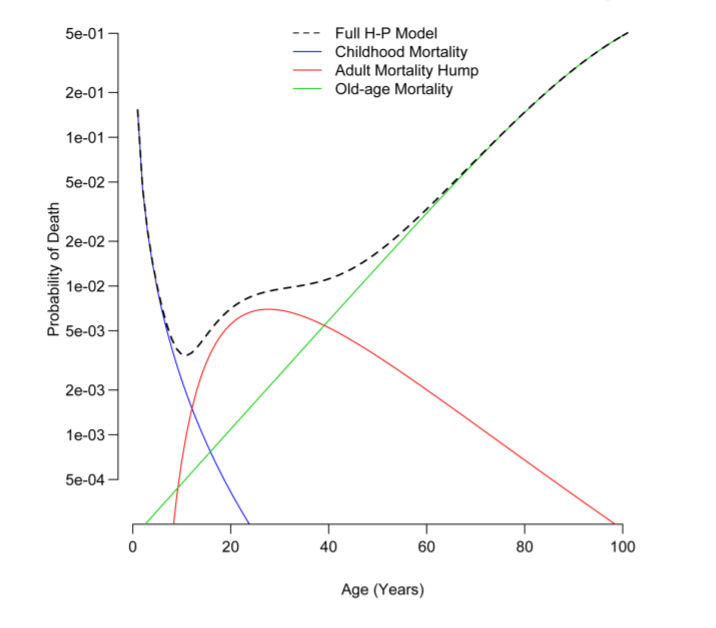
\includegraphics[height=0.7\textheight]{Graphs/HP model.png}
\caption{Decomposition of the HP model \footnote[frame]{Source: \citet{sharrow2013age}}}
\end{figure}
\end{frame}

\begin{frame}
\frametitle{Mortality Models}
Alternative to parametric mortality laws, several model life table systems have also been developed and widely used, such as the Coale-Demeny family \citep{coale1966regional}. Some organisations have also produced their own life table system, e.g. UN, GBD. 
\\~\\
These systems often use a few summary indices such as the child mortality $_5q_0$ , life expectancy at birth $\mathring{e}_0$, adult mortality $_{45}q_{15}$ etc. to generate full mortality schedules.
\end{frame}

\begin{frame}
\frametitle{Mortality Models}
A more recent model life table system is developed by \citet{wilmoth2012flexible} which has 2 parameters, namely the Log Quadratic (LogQuad) model (still somehow parameteric I guess...):
\begin{align*}
\log(m_x) = a_x + b_x \, h + c_x \, h^2 + v_x \, k,
\end{align*}
where $a_x$, $b_x$, $c_x$ and $v_x$ are constants derived from a set of life tables using SVD and $h$ and $k$ are the 2 effective parameters to vary. In addition, $h = \log(_5q_0)$, therefore given a fixed level of child mortality, a full schedule can be generated.
\end{frame}

\begin{frame}
\frametitle{Life Tables}
\begin{columns}
\column{0.5\linewidth}
\begin{figure}
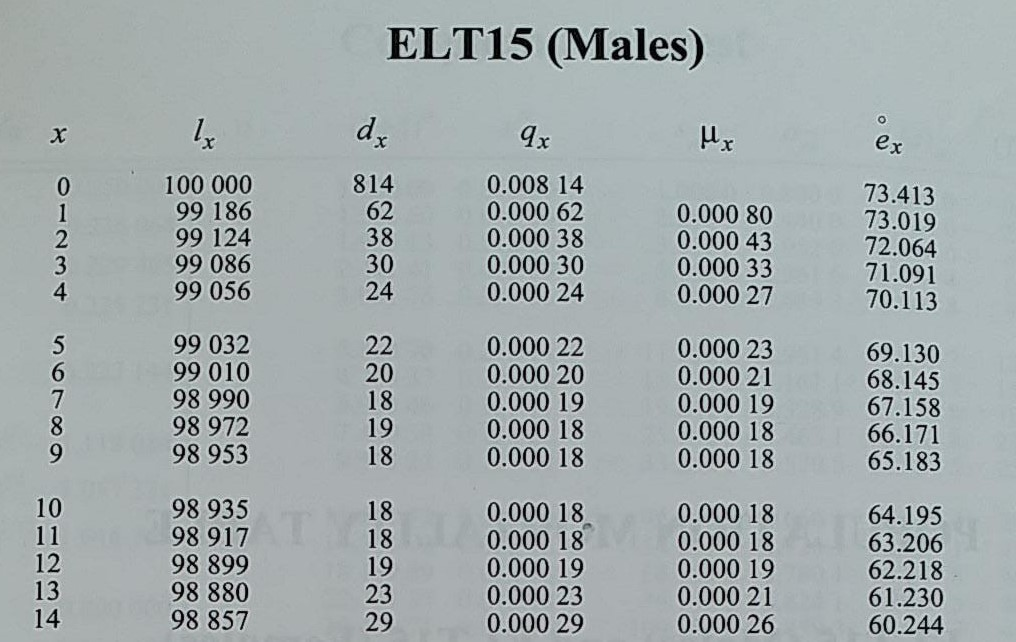
\includegraphics[width=0.95\linewidth]{Graphs/ELT15 snap.jpeg}
\caption{English Life Table 15 males \footnote[frame]{Source: Formulae and Tables for The Institute and Faculty of Actuaries}}
\end{figure}
\column{0.7\linewidth}
\begin{figure}
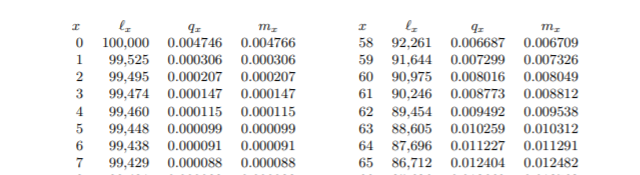
\includegraphics[width=1.2\linewidth]{Graphs/ELT17 males snap.png}
\caption{English Life Table 17 males \footnote[frame]{Source: \citet{dodd2018smoothing}}}
\end{figure}
\end{columns}
\\~\\
\begin{itemize}
\item information included may vary from tables to tables
\item columns can be derived from each other
\end{itemize}
\end{frame}

\begin{frame}
\frametitle{Bayesian Population Reconstruction}
Two main approaches:
\begin{itemize}
\item prospective reconstruction (``inverse projection'')
	\begin{itemize}
	\item[\hookrightarrow] start with a ``baseline population'' at the initial time period and project and reconstruct the population forward with corresponding demographics rates
	\end{itemize}
\item retrospective reconstruction (``back projection'')
	\begin{itemize}
	\item[\hookrightarrow] start with a final population at the terminal time period and propagate backwards in time
	\item[\hookrightarrow] however, there was debates about the efficacy of this approach as it is \textit{`trying to ``resurrect'' members of the open ended age group and simultaneously estimate fertility, mortality and migration rates.'} \citep{wheldon2016bayesian}
	\end{itemize}
\end{itemize}
\end{frame}


\begin{frame}
\frametitle{Bayesian Population Reconstruction}
I will be adopting the Bayesian population reconstruction framework by \citet{wheldon2016bayesian}
\begin{itemize}
\item prospective approach
\item Bayesian approach, gives associated uncertainty ranges of the reconstructed population counts
\end{itemize}

The core of this framework is the cohort component method of population projection (CCMPP) which utilises the concept of the demographic balancing equation
\begin{align*}
\underbrace{N_{t+1}}_{\substack{\text{population at} \\ \text{time $t+1$}}} = \underbrace{N_t}_{\substack{\text{population at} \\ \text{time $t$}}} - \underbrace{D_t}_{\text{deaths in period } t} + \underbrace{B_t}_{\text{births in period } t} + \underbrace{G_t}_{\text{net migration in period } t}
\end{align*}
\begin{itemize}
\item continuous process, need to discretise time steps
\item population projected along the cohort direction
\end{itemize}
\end{frame}

\begin{frame}
\frametitle{CCMPP}
\begin{tikzpicture}[main/.style = {draw=blue, rectangle, inner ysep=3pt,inner xsep=3pt, minimum width= 20mm},
										empty/.style = {rectangle, inner ysep=3pt,inner xsep=3pt, minimum width= 20mm}] 

\node[empty](b1){$\phantom{B_{t}}$};
\node[main, right=2cm of b1](b2){$B_{t+1}$};
\node[main, right=2cm of b2](b3){$B_{t+2}$};

\node[main, below=1.5cm of (b1)] (01) {$N_{0, t}$};
\node[main, right=2cm of 01] (02) {$N_{0, t+1}$};
\node[main, right=2cm of 02] (03) {$N_{0, t+2}$};

\node[main, below=1.5cm of 01](11){$N_{x,t}$};
\node[main, below=0cm of 11](21){$N_{x+1,t}$};

\node[main, right=2cm of 21](12){$N_{x+1,t+1}$};
\node[main, below=0cm of 12](22){$N_{x+2,t+1}$};

\node[main, right=2cm of 22](13){$N_{x+2,t+2}$};
\node[main, below=0cm of 13](23){$N_{x+3,t+2}$};

\node[main, below=2cm of 21](end1){$N_{oag-1,t}$};
\node[main, below=0cm of end1](oag1){$N_{oag,t}$};

\node[main, right=2cm of end1](end2){$N_{oag-1,t+1}$};
\node[main, below=0cm of end2](oag2){$N_{oag,t+1}$};
\node[main, right=2cm of end2](end3){$N_{oag-1,t+2}$};
\node[main, below=0cm of end3](oag3){$N_{oag,t+2}$};

\path(01)--(11) node[empty, midway](1dots1) {$\vdots$};
\path(21)--(end1) node[empty, midway](2dots1) {$\vdots$};
\path(02)--(12) node[empty, midway](1dots2) {$\vdots$};
\path(22)--(end2) node[empty, midway](2dots2) {$\vdots$};
\path(03)--(13) node[empty, midway](1dots3) {$\vdots$};
\path(23)--(end3) node[empty, midway](2dots3) {$\vdots$};

\draw[thick, ->] (11)--(12);
\draw[thick, ->] (21)-- node[below left]{$\boldsymbol{s}_{x,t}$}(22);
\draw[thick, ->] (12)--(13);
\draw[thick, ->] (22)-- node[below]{$\boldsymbol{s}_{x,t+1}$}(23);

\draw[thick, ->] (end1)--(oag2);
\draw[thick, ->] (oag1)-- node[below]{$s_{oag,t}$}(oag2);
\draw[thick, ->] (end2)--(oag3);
\draw[thick, ->] (oag2)-- node[below]{$s_{oag,t+1}$}(oag3);

\draw[thick, ->] (01)--(1dots2);
\draw[thick, ->] (02)--(1dots3);

\draw[thick, ->] (b2)-- node[left]{$s_{0^-,t+1}$}(02);
\draw[thick, ->] (b3)-- node[left]{$s_{0^-,t+2}$}(03);

\draw[red, thick, ->](1dots1) to [out=0, in =-180, looseness=1.3, "{$\boldsymbol{f}_{x,t}$}"] (b2);
\draw[red, thick, ->](11) to [out=0, in =-178, looseness=1.3] (b2);
\draw[red, thick, ->](21) to [out=0, in =-175, looseness=1.2] (b2);
\draw[red, thick, ->](2dots1) to [out=5, in =-172, looseness=1] (b2);

\draw[red, thick, ->](1dots2) to [out=0, in =-180, looseness=1.2, "{$\boldsymbol{f}_{x,t+1}$}"] (b3);
\draw[red, thick, ->](12) to [out=0, in =-178, looseness=1.1] (b3);
\draw[red, thick, ->](22) to [out=0, in =-175, looseness=1] (b3);
\draw[red, thick, ->](2dots2) to [out=5, in =-172, looseness=0.8] (b3);

\draw[black!35!green, thick, ->](01) -- (02);
\draw[black!35!green, thick, ->](01) to [bend left=5] (1dots2);
\draw[black!35!green, thick, ->](11) to [bend left=5] node[above right]{$\boldsymbol{g}_{x,t}$} (12);
\draw[black!35!green, thick, ->](21) -- (12);
\draw[black!35!green, thick, ->](21) to [bend left=5] (22);
\draw[black!35!green, thick, ->](2dots1) to [bend left=5] (22);

\draw[black!35!green, thick, ->](02) -- (03);
\draw[black!35!green, thick, ->](02) to [bend left=5] (1dots3);
\draw[black!35!green, thick, ->](12) to [bend left=5] node[above right]{$\boldsymbol{g}_{x,t+1}$} (13);
\draw[black!35!green, thick, ->](22) -- (13);
\draw[black!35!green, thick, ->](22) to [bend left=5] (23);
\draw[black!35!green, thick, ->](2dots2) to [bend left=5] (23);

\draw[black!35!green, thick, ->](end1) -- (end2);
\draw[black!35!green, thick, ->](end1) to [bend left=5] (oag2);
\draw[black!35!green, thick, ->](oag1) to [bend right=5] (oag2);
\draw[black!35!green, thick, ->](end2) -- (end3);
\draw[black!35!green, thick, ->](end2) to [bend left=5] (oag3);
\draw[black!35!green, thick, ->](oag2) to [bend right=5] (oag3);

\end{tikzpicture}
\end{frame}

\begin{frame}
\frametitle{Bayesian Population Reconstruction}
Require demographics rates (fertility rates, survival proportions, net migration proportions) to project the populations
\begin{align*}
N^*_{x,\color{red}t_0}|\sigma^2_N \quad &\sim \quad logNormal(\log(N_{x,\color{red}t_0}), \sigma^2_N) \\
f^*_{x,t}|\sigma^2_f \quad & \sim \quad logNormal(\log(f_{x,t}), \sigma^2_f) \quad \forall x \in [15, 50) \\
s^*_{x,t}|\sigma^2_s \quad & \sim \quad logNormal(\log(s_{x,t}), \sigma^2_s) \\
g^*_{x,t}|\sigma^2_g \quad &\sim \quad AR1:AR1(\rho_x, \rho_t, \sigma^2_g) \\
N^*_{x,t} | f^*_{x,t}, s^*_{x,t}, g^*_{x,t} \quad & \, \, \textcolor{red}{=} \quad CCMPP(N^*_{x,\color{red}t_0}, f^*_{x,t}, s^*_{x,t}, g^*_{x,t}, srb) \quad \forall t \neq t_0 \\
N_{x,t} \quad &\sim \quad logNormal(\log(\textcolor{red}{N^*_{x,t}}), \sigma^2_N) \quad \forall t \neq t_0 \\
\sigma^2_N, \sigma^2_f, \sigma^2_s, \sigma^2_g, \rho_x, \rho_t \quad &\propto  \quad h(\cdot)
\end{align*}
\end{frame}

\begin{frame}
\frametitle{Bayesian Population Reconstruction}
Instead of using estimates of the survival proportions from other data source as priors, incorporate DHS data into population reconstruction
\begin{itemize}
\item DHS data supports estimation of mortality rates $m_x$, and most models are on $m_x$ instead of survival proportions $s_x$
 \begin{itemize}
 \item[\hookrightarrow] convert $m_x$ to $s_x$
 \end{itemize}
\item DHS data limited age range (15 - 60), where as population reconstruction spans the full age range (0 - open age group)
 \begin{itemize}
 \item[\hookrightarrow] utilise laws of mortality / model life tables, e.g. LogQuad, HP-8, Thiele
 \end{itemize}
\end{itemize}
\end{frame}


\begin{frame}
\frametitle{Conversion between $m_x$ and $s_x$}
$s_x$, the survivorship between age groups, are then calculated by $\frac{L_{x+1}}{L_{x}}$, where $L_x$ denotes the exposures in the period at age $[x, x+1)$. Under UDD, $L_x = l_x - \frac{1}{2} d_x$,
\begin{align*}
s_x &\stackrel{\smash{\scriptscriptstyle\mathrm{UDD}}}{=} \tensor[_{0.5}]{p}{_{x+0.5}} \, \, \tensor[_{0.5}]{p}{_{x+1}} \\
	& \, \, = \tensor[_{\phantom{0.}1}]{p}{_{x+0.5}}
\end{align*}
\end{frame}

\begin{frame}
\frametitle{Open Age Group Mortality Rate}
Aggregating mortality rates of the last age groups into an open age group also needs attention.

\begin{align*}
m_{oag} &= \frac{\sum_{i \geq oag} w_i m_i }{\sum_{i \geq oag} w_i}
\end{align*}
where, under UDD,
\begin{align*}
w_i &= (1-0.5 \, q_i) \prod_{oag \leq \, j \, < i} p_j
\end{align*}
\end{frame}

\begin{frame}
\frametitle{LogQuad Model - Females}
Using IGME child moratlity estimates as priors for the LogQuad parameters
\begin{columns}
\column{0.5\linewidth}
\begin{figure}
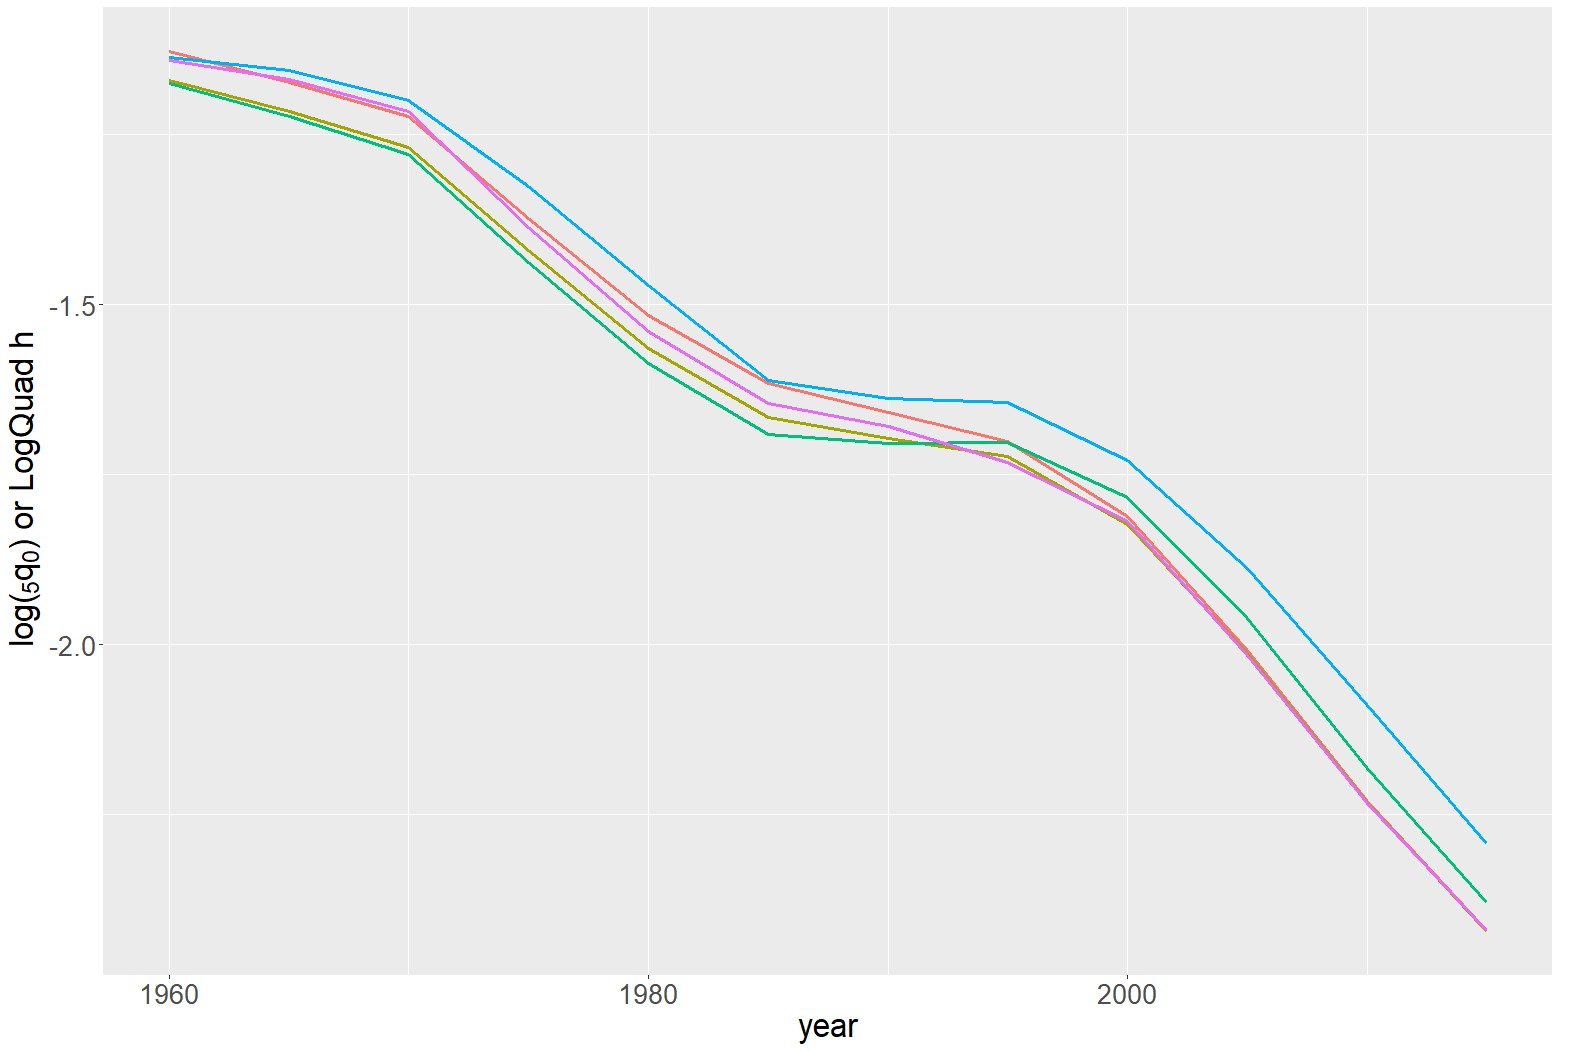
\includegraphics[width=\linewidth]{Graphs/female h.jpg}
\caption{Estimated log child mortality. \\IGME estimates in red.}
\end{figure}
\column{0.5\linewidth}
\begin{figure}
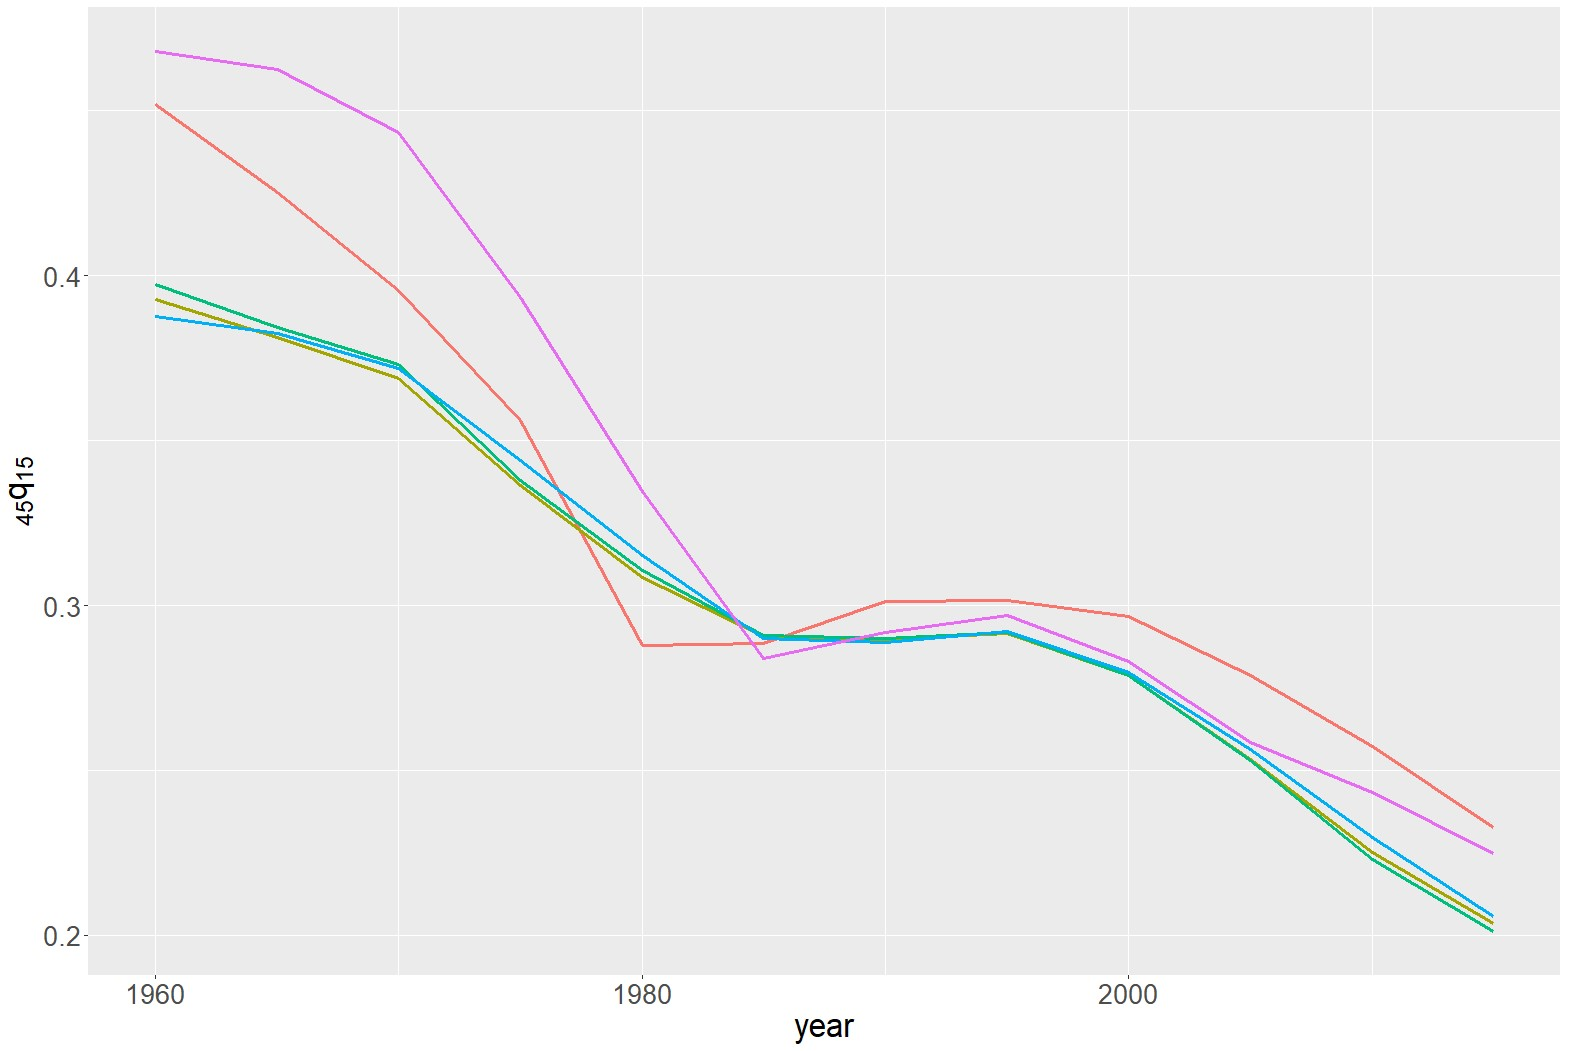
\includegraphics[width=\linewidth]{Graphs/female q4515.jpg}
\caption{Estimated $_{45}q_{15}$. \\WPP estimates in red.}
\end{figure}
\end{columns}
\end{frame}

\begin{frame}
\frametitle{LogQuad Model - Joint Sex}
\begin{columns}
\column{0.5\linewidth}
\begin{figure}
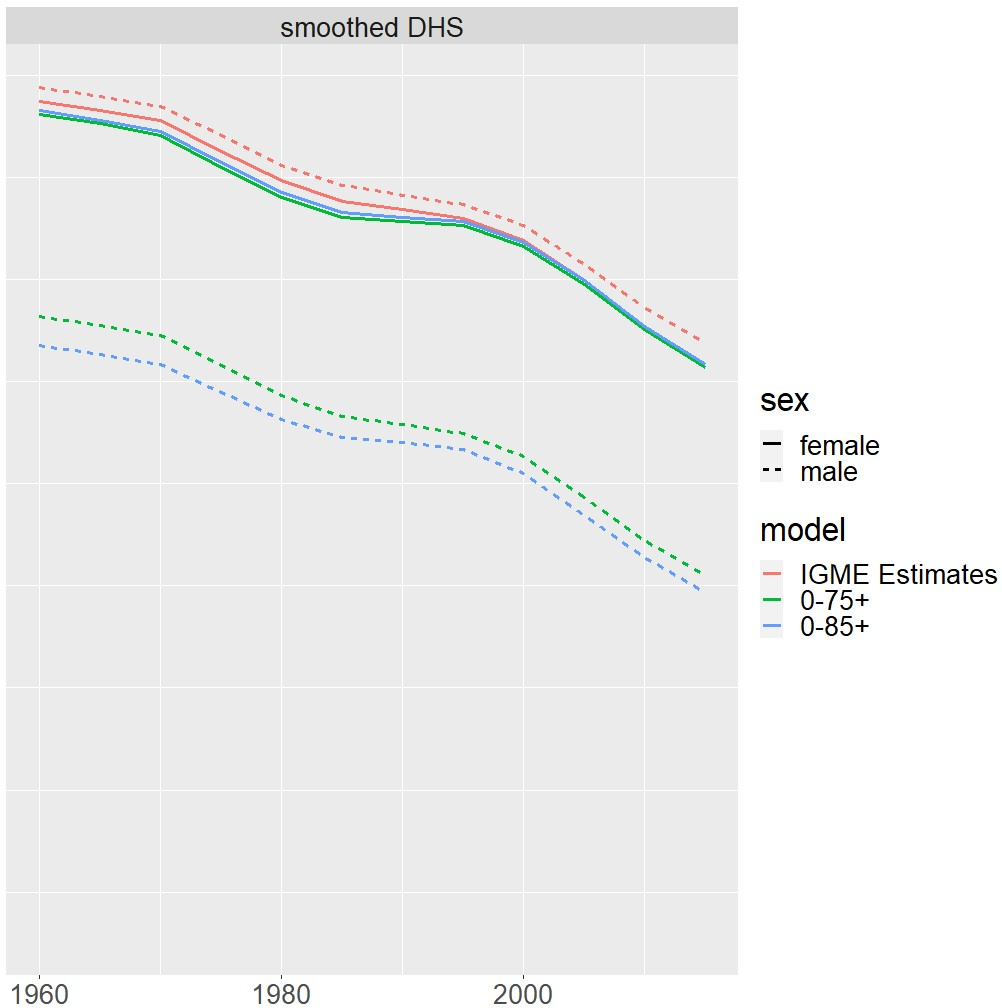
\includegraphics[width=\linewidth]{Graphs/joint h.jpg}
\caption{Estimated log child mortality. \\IGME estimates in red.}
\end{figure}
\column{0.5\linewidth}
\begin{itemize}
\item Estimated male child mortality is much lower than the IGME estimates
\item LogQuad developed for countries without HIV
\item HIV-hump in mortality in adult ages (age range with DHS data) affects estimated child mortality due to the in-flexibility of the LogQuad model for HIV-infected populations
\end{itemize}
\end{columns}
\end{frame}


\begin{frame}
\frametitle{LogQuad Model - Zimbabwe}
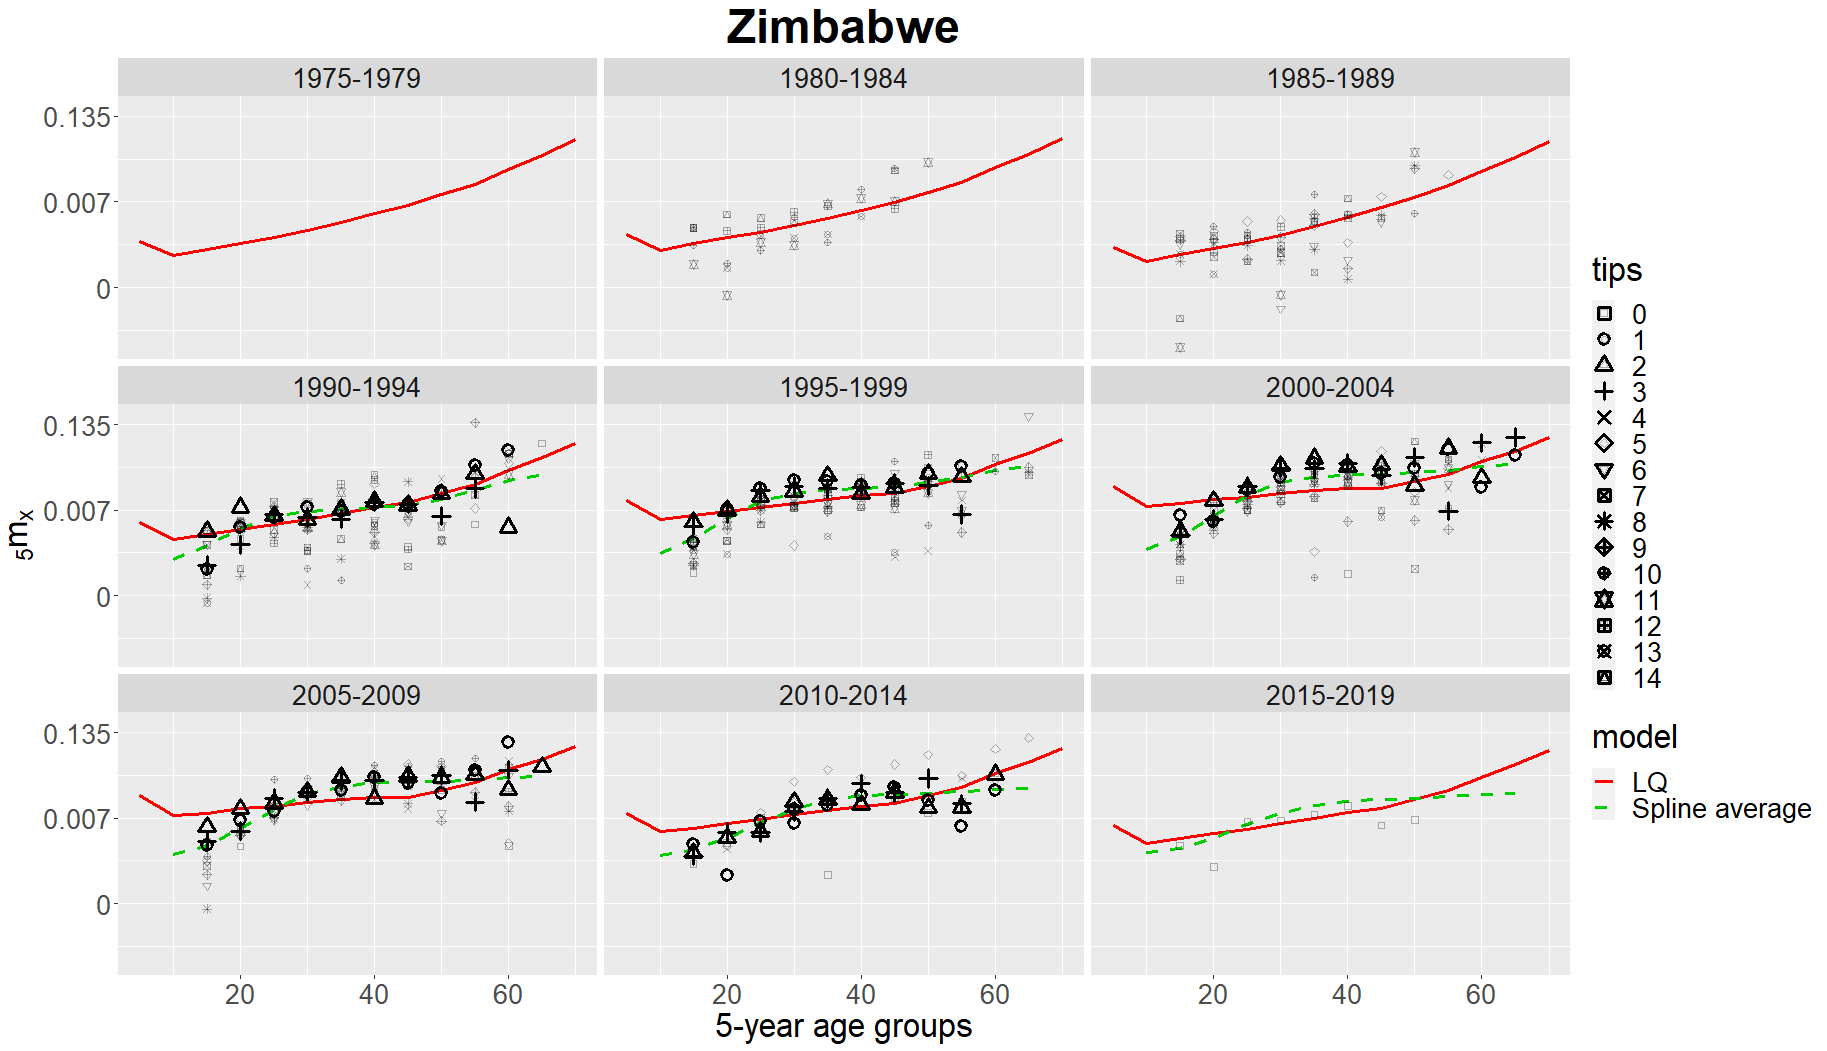
\includegraphics[width=\linewidth]{Graphs/Zimbabwe LQ female.png}
LQ obviously not meant for naive implementation in high-HIV countries, but this illustrates the LQ fit in this context
\end{frame}

\begin{frame}
\frametitle{LogQuad Model + DEF Hump from the HP-8 Model}
Recall the HP-8 Model decomposes the age pattern into 3 stages
\begin{equation*}
	\frac{q_x}{1-q_x} = A^{(x + B)^C} + D e^{-E(ln x - ln F)^2} + GH^x,
\end{equation*}

Attempted to extract the middle hump and add it on top of the LQ model and fit only to the DHS data, still using IGME estimates as priors.
\end{frame}

\begin{frame}
\frametitle{LogQuad Model + DEF Hump from the HP-8}
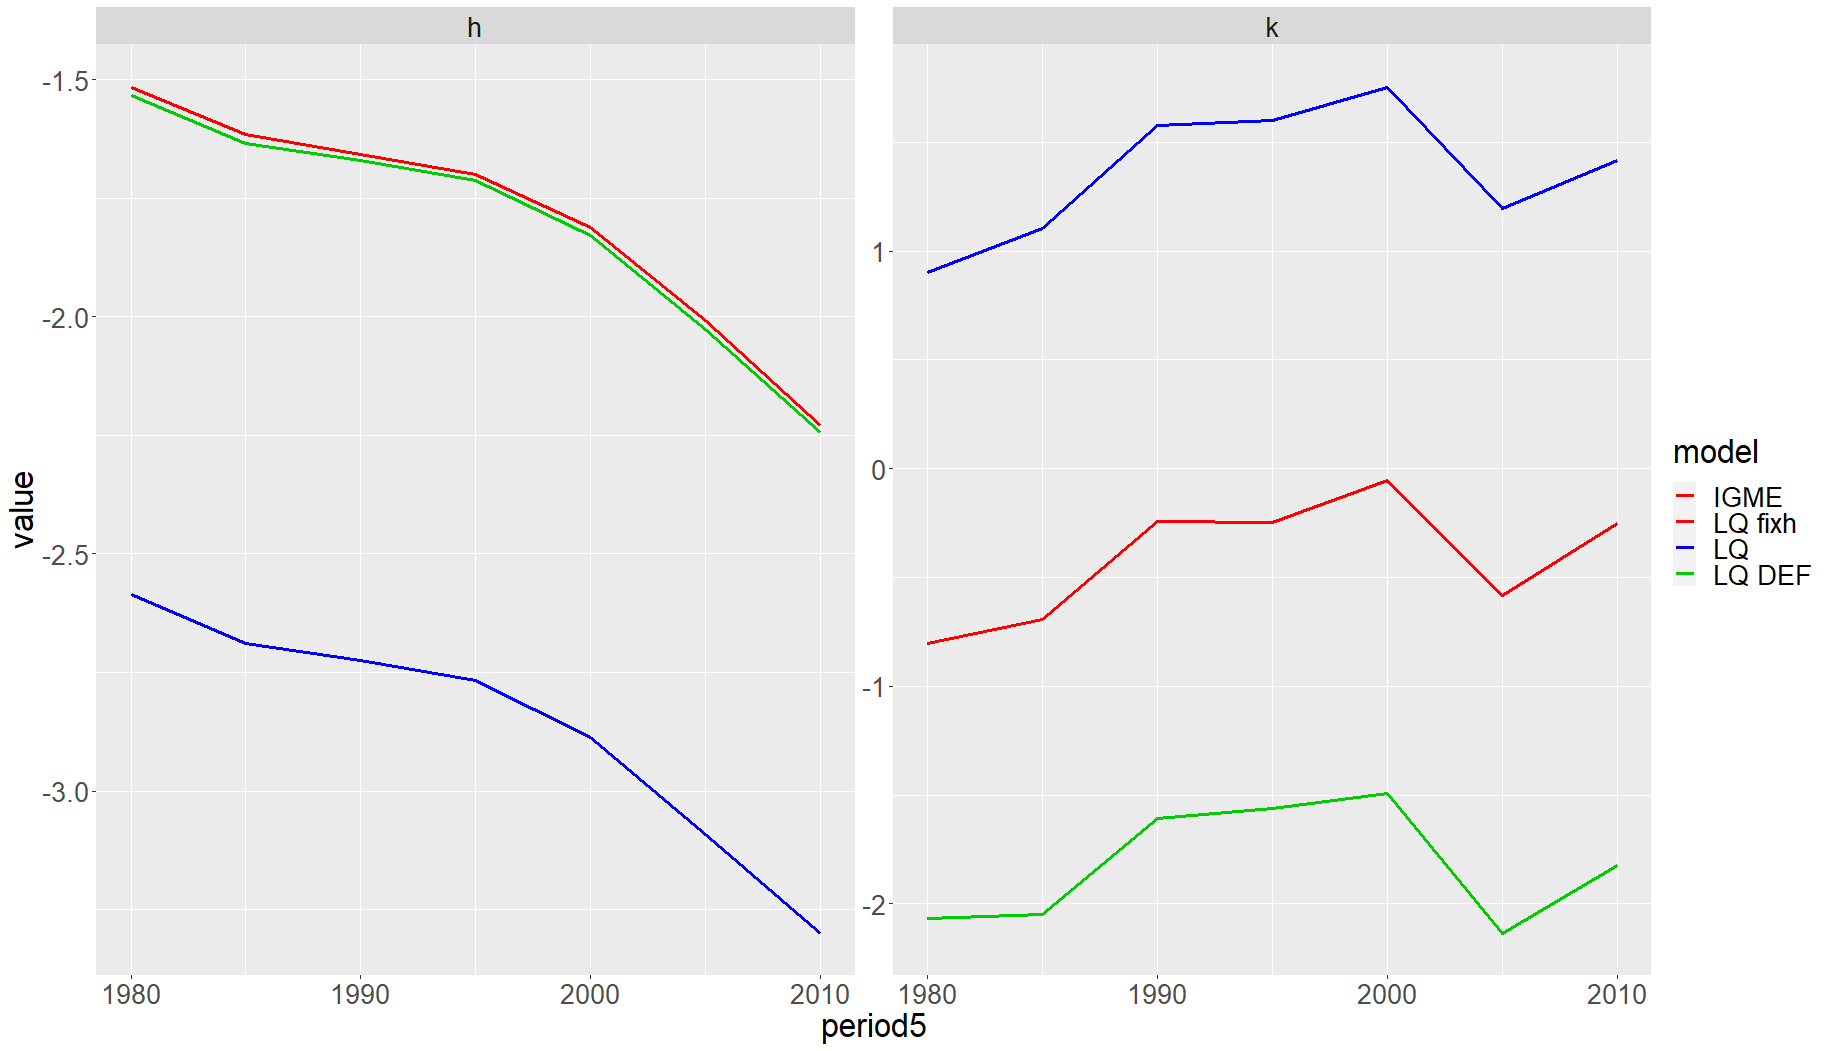
\includegraphics[scale=0.18]{Graphs/fix DEF hk males.png}

\begin{itemize}
\item LQ+DEF allows the estimated child mortality to be more consistent for males (green and red)
\item difficult to converge for females and gives insensible results, possibly due to the less prominent hump in Burkina Faso as well as the corerlation between the DEF and the LQ $k$
\end{itemize}
\end{frame}


\begin{frame}
\frametitle{Thiele}

 \begin{align*}
m(x) = \underbrace{\varphi e^{-\psi x}}_\text{negative exponential} + \, \underbrace{\lambda e^{-\delta (x-\epsilon)^2}}_\text{normal}+ \underbrace{A e^{B x}}_\text{Gompertz} \qquad \varphi,\psi,\lambda,\delta,\epsilon > 0
 \end{align*}

Used IGME estimates and LogQuad model to derive priors for the 7 parameters of Thiele
\begin{itemize}
\item consistent child mortality estimates with the IGME estimates
\item sensible results
\item converged quite stably for different countries (so far)
\end{itemize}
\end{frame}


\begin{frame}
\frametitle{Thiele}
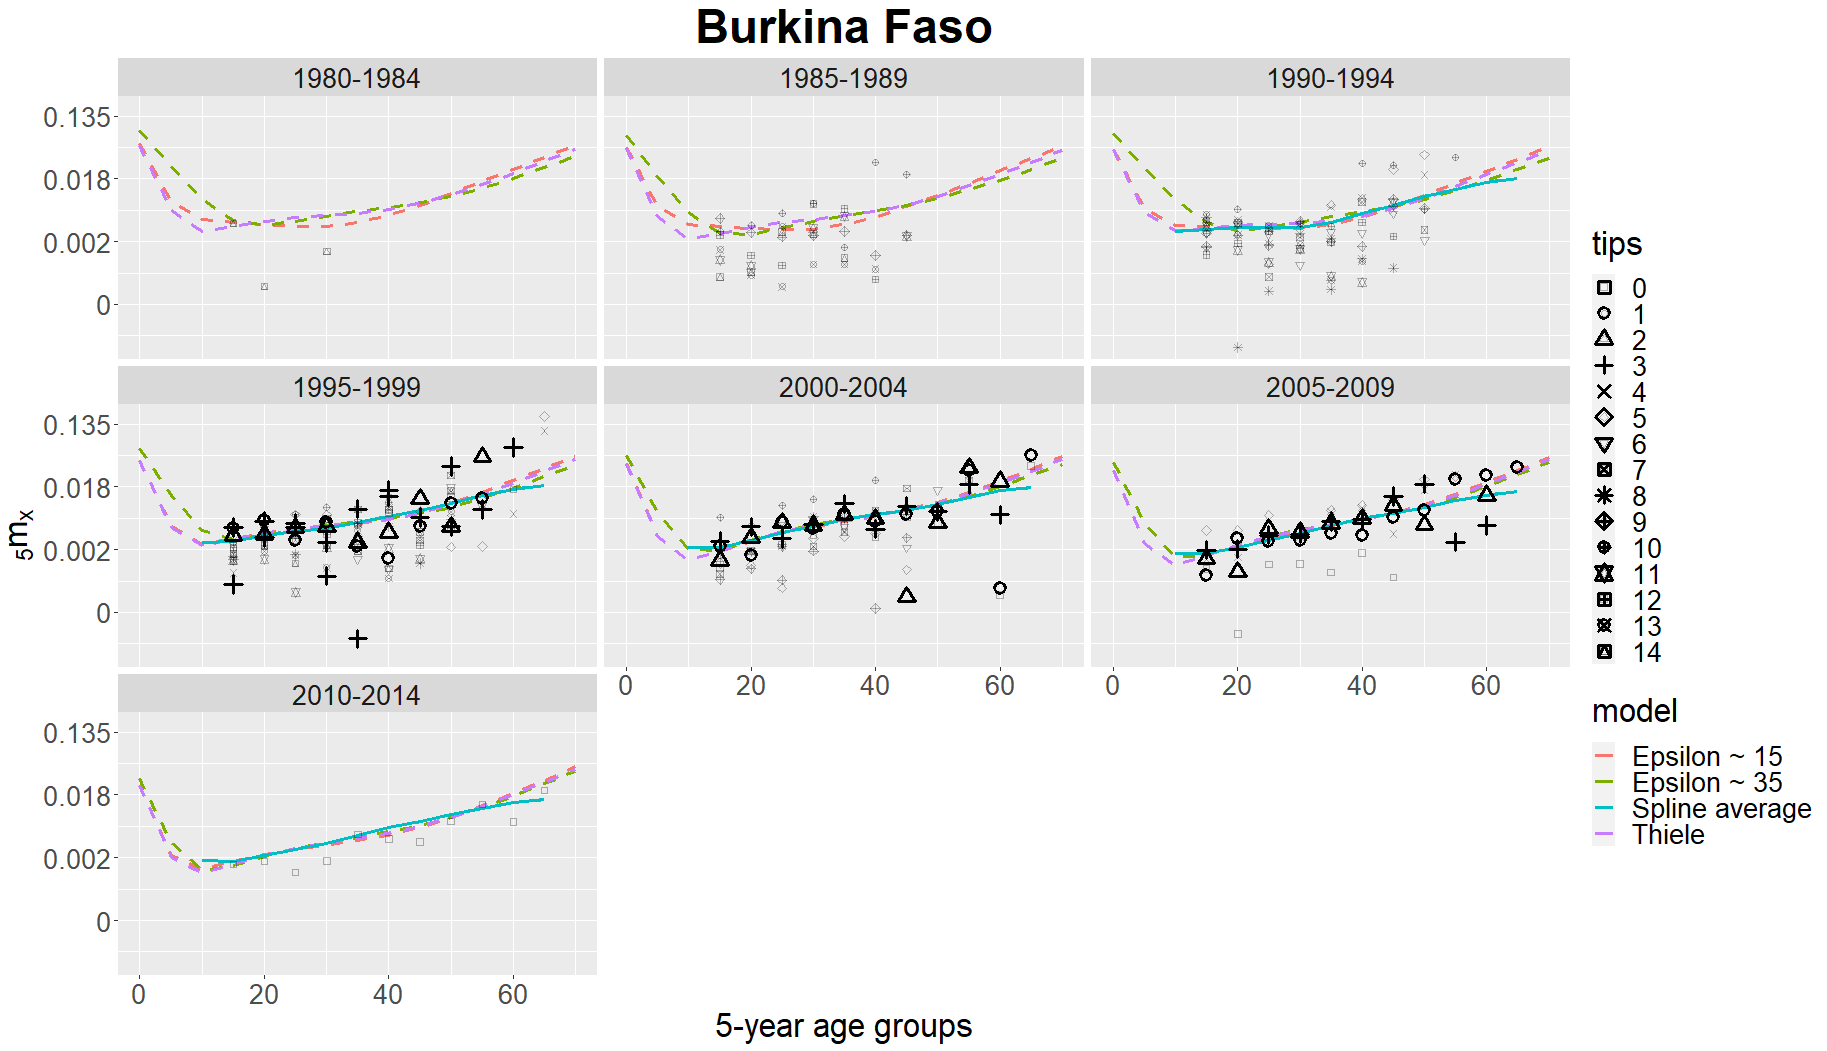
\includegraphics[width=\linewidth]{Graphs/Thiele female.png}
\end{frame}

\begin{frame}
\frametitle{Thiele}
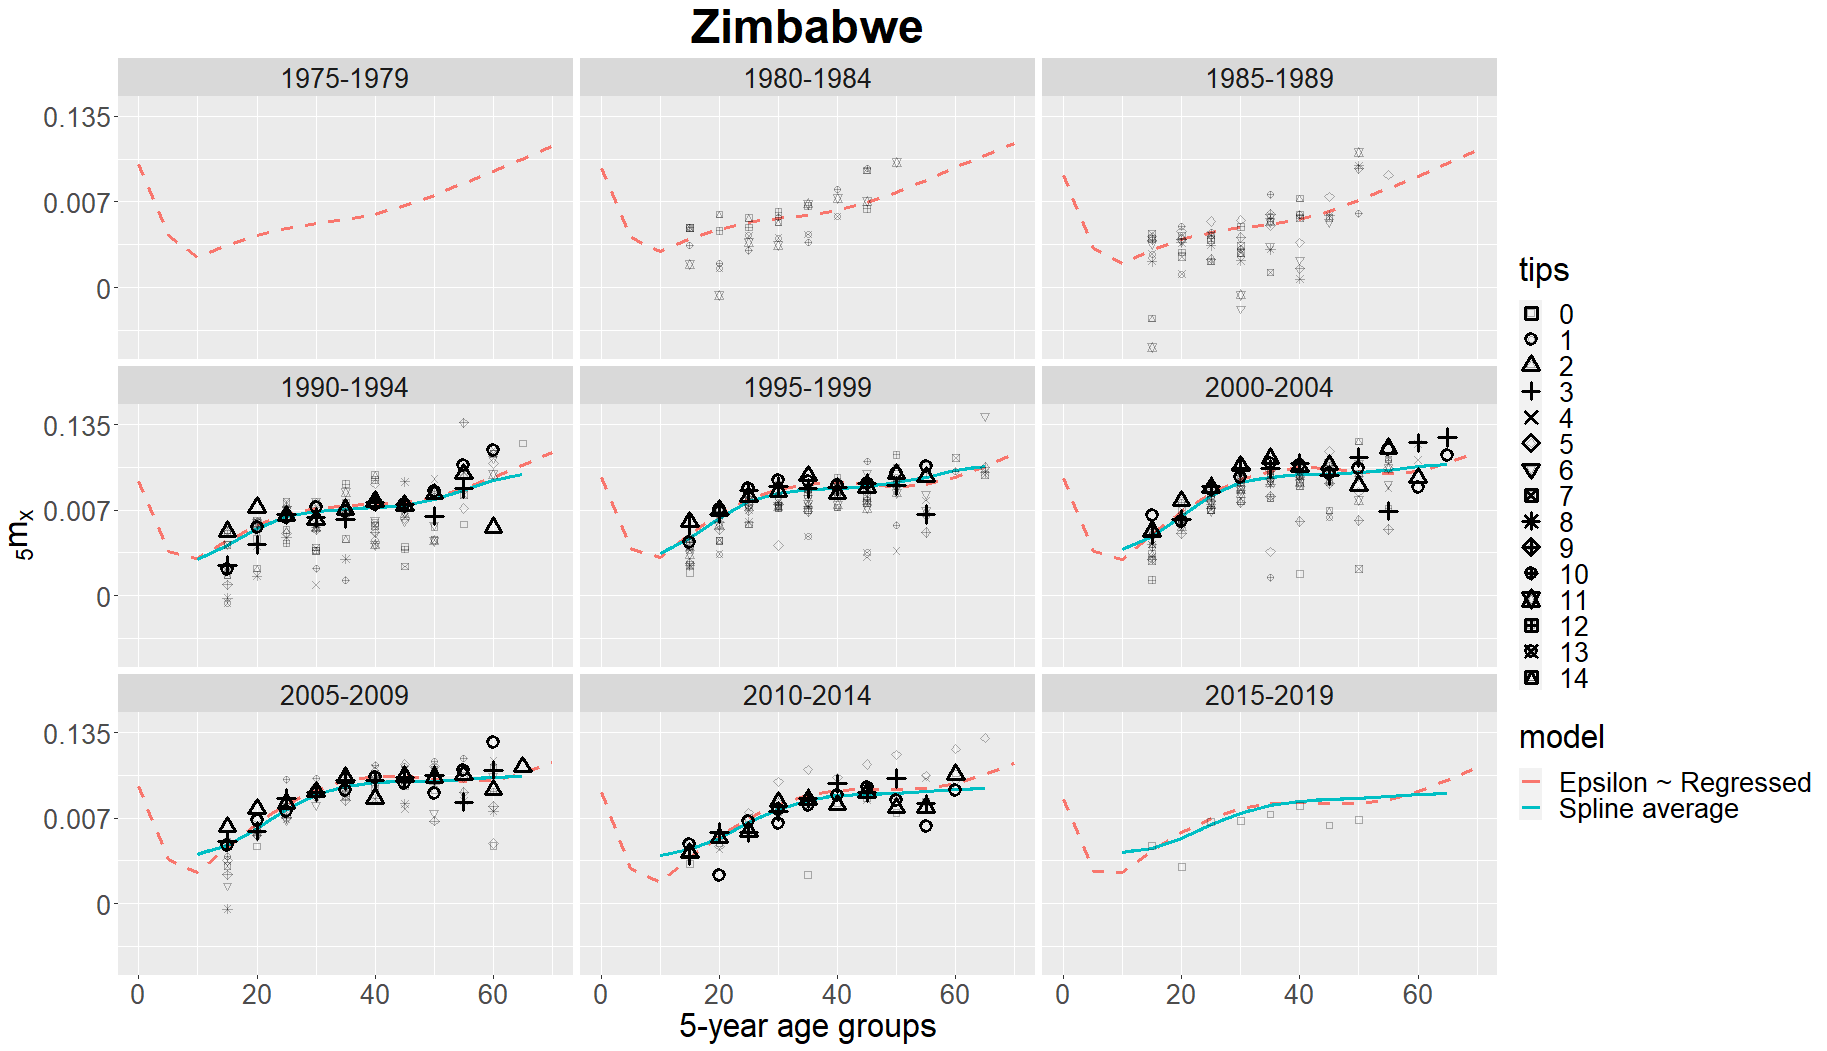
\includegraphics[width=\linewidth]{Graphs/Zimbabwe female.png}
Adequate fit even to high HIV countries
\end{frame}

\begin{frame}
\frametitle{Thiele}
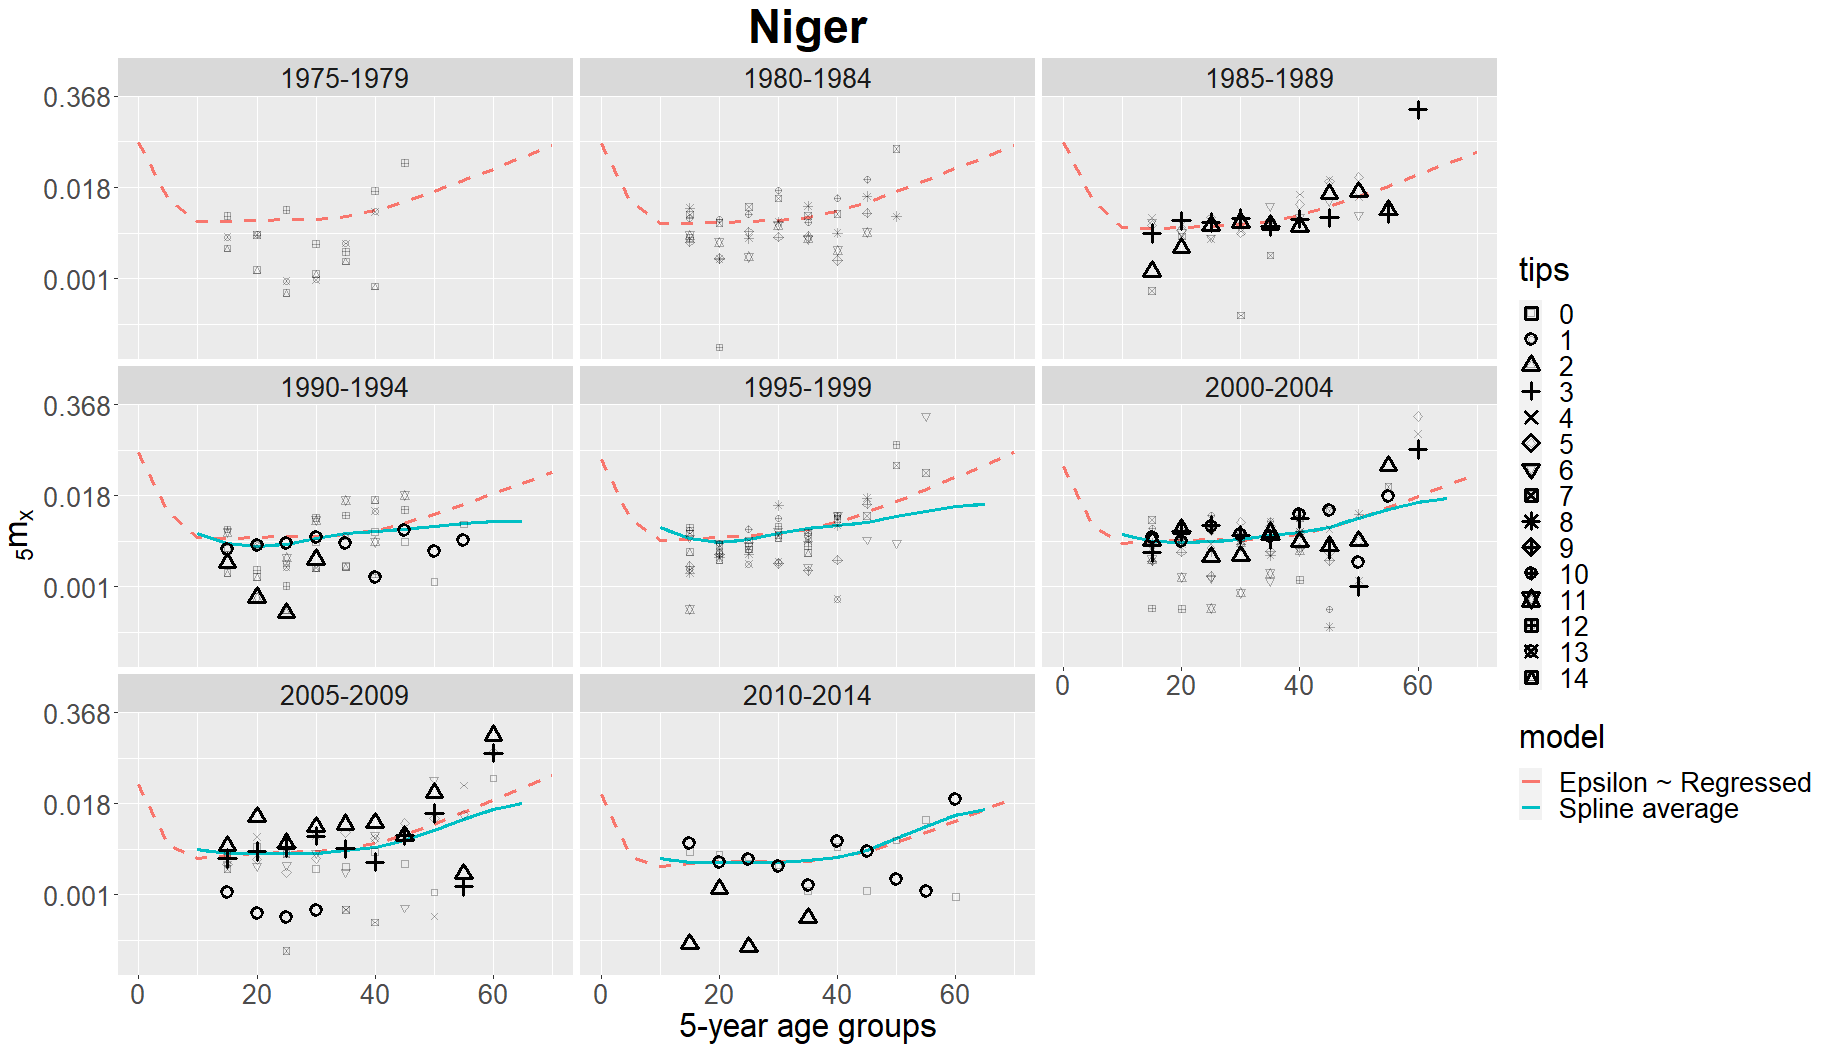
\includegraphics[width=\linewidth]{Graphs/Niger female.png}
Also in very low HIV countries
\end{frame}

\begin{frame}
\frametitle{Thiele}
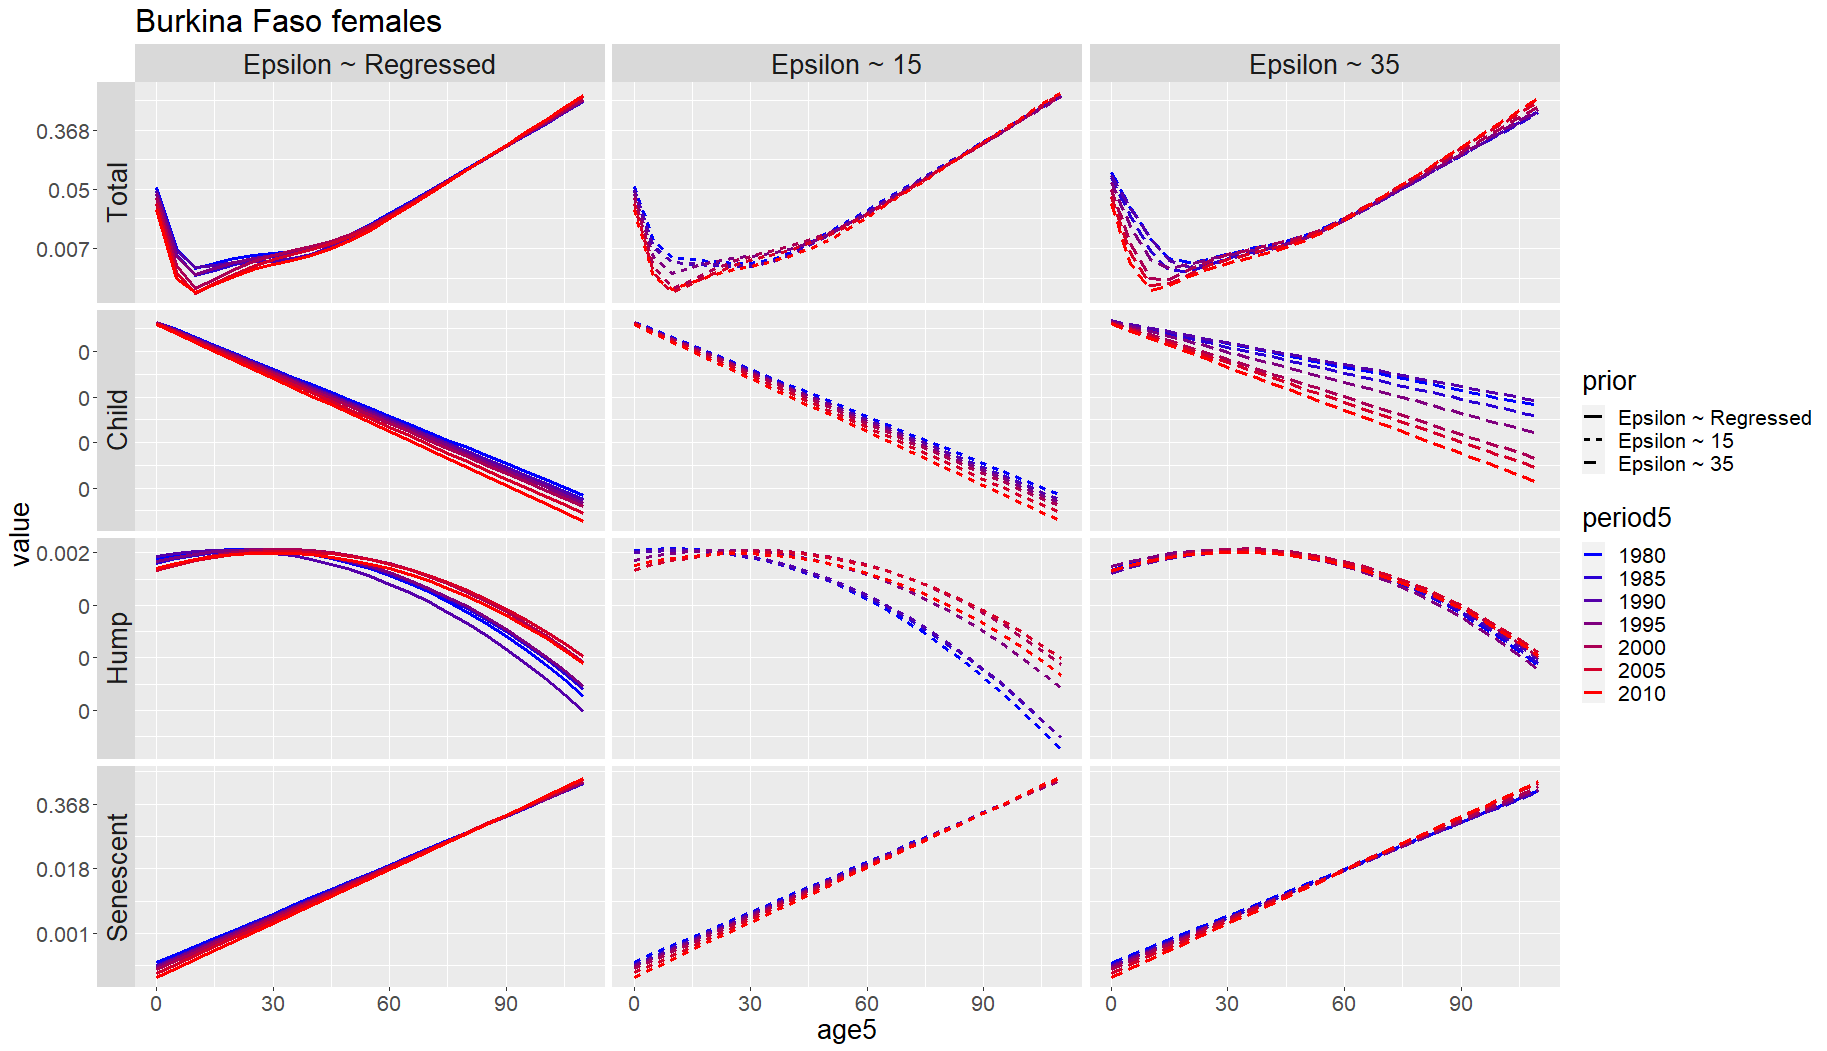
\includegraphics[width=\linewidth]{Graphs/Thiele female decomp.png}
Thiele estimated $m_x$ and decomposed
\end{frame}

\begin{frame}
\frametitle{Next Steps}
\begin{itemize}
\item So far, because of the issues encountered with the LogQuad model, took a step back and modelled only DHS data
\item Incorporate Thiele model into population reconstruction
\item Try to modify the hump component of the model such that it is on log-scale and compare fit
\item Extend to other countries
\end{itemize}
\end{frame}

\bibliographystyle{apalike}
\bibliography{Ref}

\end{document}